\newpage

\section{ПОСТАНОВКА ЗАДАЧИ}

% = = = = =

\subsection{Перечень функций}

Достижение цели курсовой работы предполагает необходимость создания приложения
для работы с локальной базой данных на тему <<Товары>> с использованием пользовательского
интерфейса и решения следующих конкретных задач:

\begin{enumerate}
    \item добавление товара в базу данных;
    \item вывод товаров из базы данных;
    \item удаление товара из базы данных;
    \item изменение товара в базу данных;
    \item сохранение товаров из базы данных в файл JSON;
    \item сохранение товаров из базы данных в файл CSV;
    \item открытие файла JSON и добавление товаров в базу данных.
\end{enumerate}

% = = = = =

\subsection{Требования пользователей}

Пользовательские требования - описание на естественном языке (плюс поясняющие диаграммы) функций,
выполняемых системой, и ограничений, накладываемых на неё.

Источники: Пользователь

Документ: Пользовательские требования / требования к ПО.

Ответственный: Системный аналитик.

Эти требования должны определять только внешнее поведение системы,
избегая по возможности определения структурных характеристик системы.
Пользовательские требования должны быть написаны естественным языком с использованием
простых таблиц, а также наглядных и понятных диаграмм.

Требования пользователя к информационной системе:

Обязательные:

\begin{enumerate}
    \item должна быть реализована функция ввода данных в информационную систему;
    \item должна работать функция удаления записи из информационной системы.
\end{enumerate}

Желательные:

\begin{enumerate}
    \item информационная система должна выводить отчеты на печать.
\end{enumerate}

% = = = = =

\subsection{Проектирование архитектуры ПО (модули)}

Архитектура программного обеспечения (англ. software architecture) - совокупность
важнейших решений об организации программной системы.

Архитектура включает:

\begin{itemize}
    \item выбор структурных элементов и их интерфейсов, с помощью которых составлена система,
    а также их поведения в рамках сотрудничества структурных элементов
    \item соединение выбранных элементов структуры и поведения во всё более крупные системы
    \item архитектурный стиль, который направляет всю организацию - все элементы, их интерфейсы,
    их сотрудничество и их соединение.
\end{itemize}

Документирование архитектуры программного обеспечения (ПО) упрощает процесс коммуникации
между разработчиками, позволяет зафиксировать принятые проектные решения
и предоставить информацию о них эксплуатационному персоналу системы,
повторно использовать компоненты и шаблоны проекта в других.

Архитектурный вид состоит из 2 компонентов:

\begin{enumerate}
    \item [1.] Элементы
    \item [2.] Отношения между элементами
\end{enumerate}

Архитектурные виды можно поделить на 3 основных типа:

\begin{itemize}
    \item [1.] Модульные виды (англ. module views) - показывают систему как структуру
    из различных программных блоков.
    \item [2.] Компоненты-и-коннекторы (англ. component-and-connector views) - показывают
    систему как структуру из параллельно запущенных элементов (компонентов)
    и способов их взаимодействия (коннекторов).
    \item [3.] Размещение (англ. allocation views) - показывает размещение
    элементов системы во внешних средах.
\end{itemize}

Примеры модульных видов:

Декомпозиция (англ. decomposition view) - состоит из модулей в контексте
отношения <<является подмодулем>>.

Использование (англ. uses view) - состоит из модулей в контексте
отношения <<использует>> (т.е. один модуль использует сервисы другого модуля).

Вид уровней (англ. layered view) - показывает структуру,
в которой связанные по функциональности модули объединены в группы (уровни).

Вид классов/обобщений (англ. class/generalization view) - состоит из классов,
связанные через отношения <<наследуется от>> и <<является экземпляром>>.

\subsubsection*{Иерархия модулей и подмодулей разрабатываемой программы для frontend}

Информационная система включает в себя следующие модули на frontend:

\begin{itemize}
    \item модуль не найденной страницы
    \item модуль авторизации
    \item модуль выхода
    \item модуль меню
    \begin{itemize}
        \item модуль, реализующий добавление новых записей в базу данных;
        \item модуль организации локальной базы данных с выводом информации о товарах;
        \begin{itemize}
            \item модуль удаления записи из локальной базы данных;
        \end{itemize}
        \item модуль, осуществляющий изменение записи;
        \item модуль, осуществляющий сохранение данных в JSON;
        \item модуль, осуществляющий сохранение данных в CSV;
        \item модуль, осуществляющий открытие файла JSON.
    \end{itemize}
\end{itemize}

Схема frontend модулей изображена на
\textbf{рис. \ref{fig:gpi_frontend_modules} (стр. \pageref{fig:gpi_frontend_modules})}.

\begin{figure}[!htp]
    \centering
    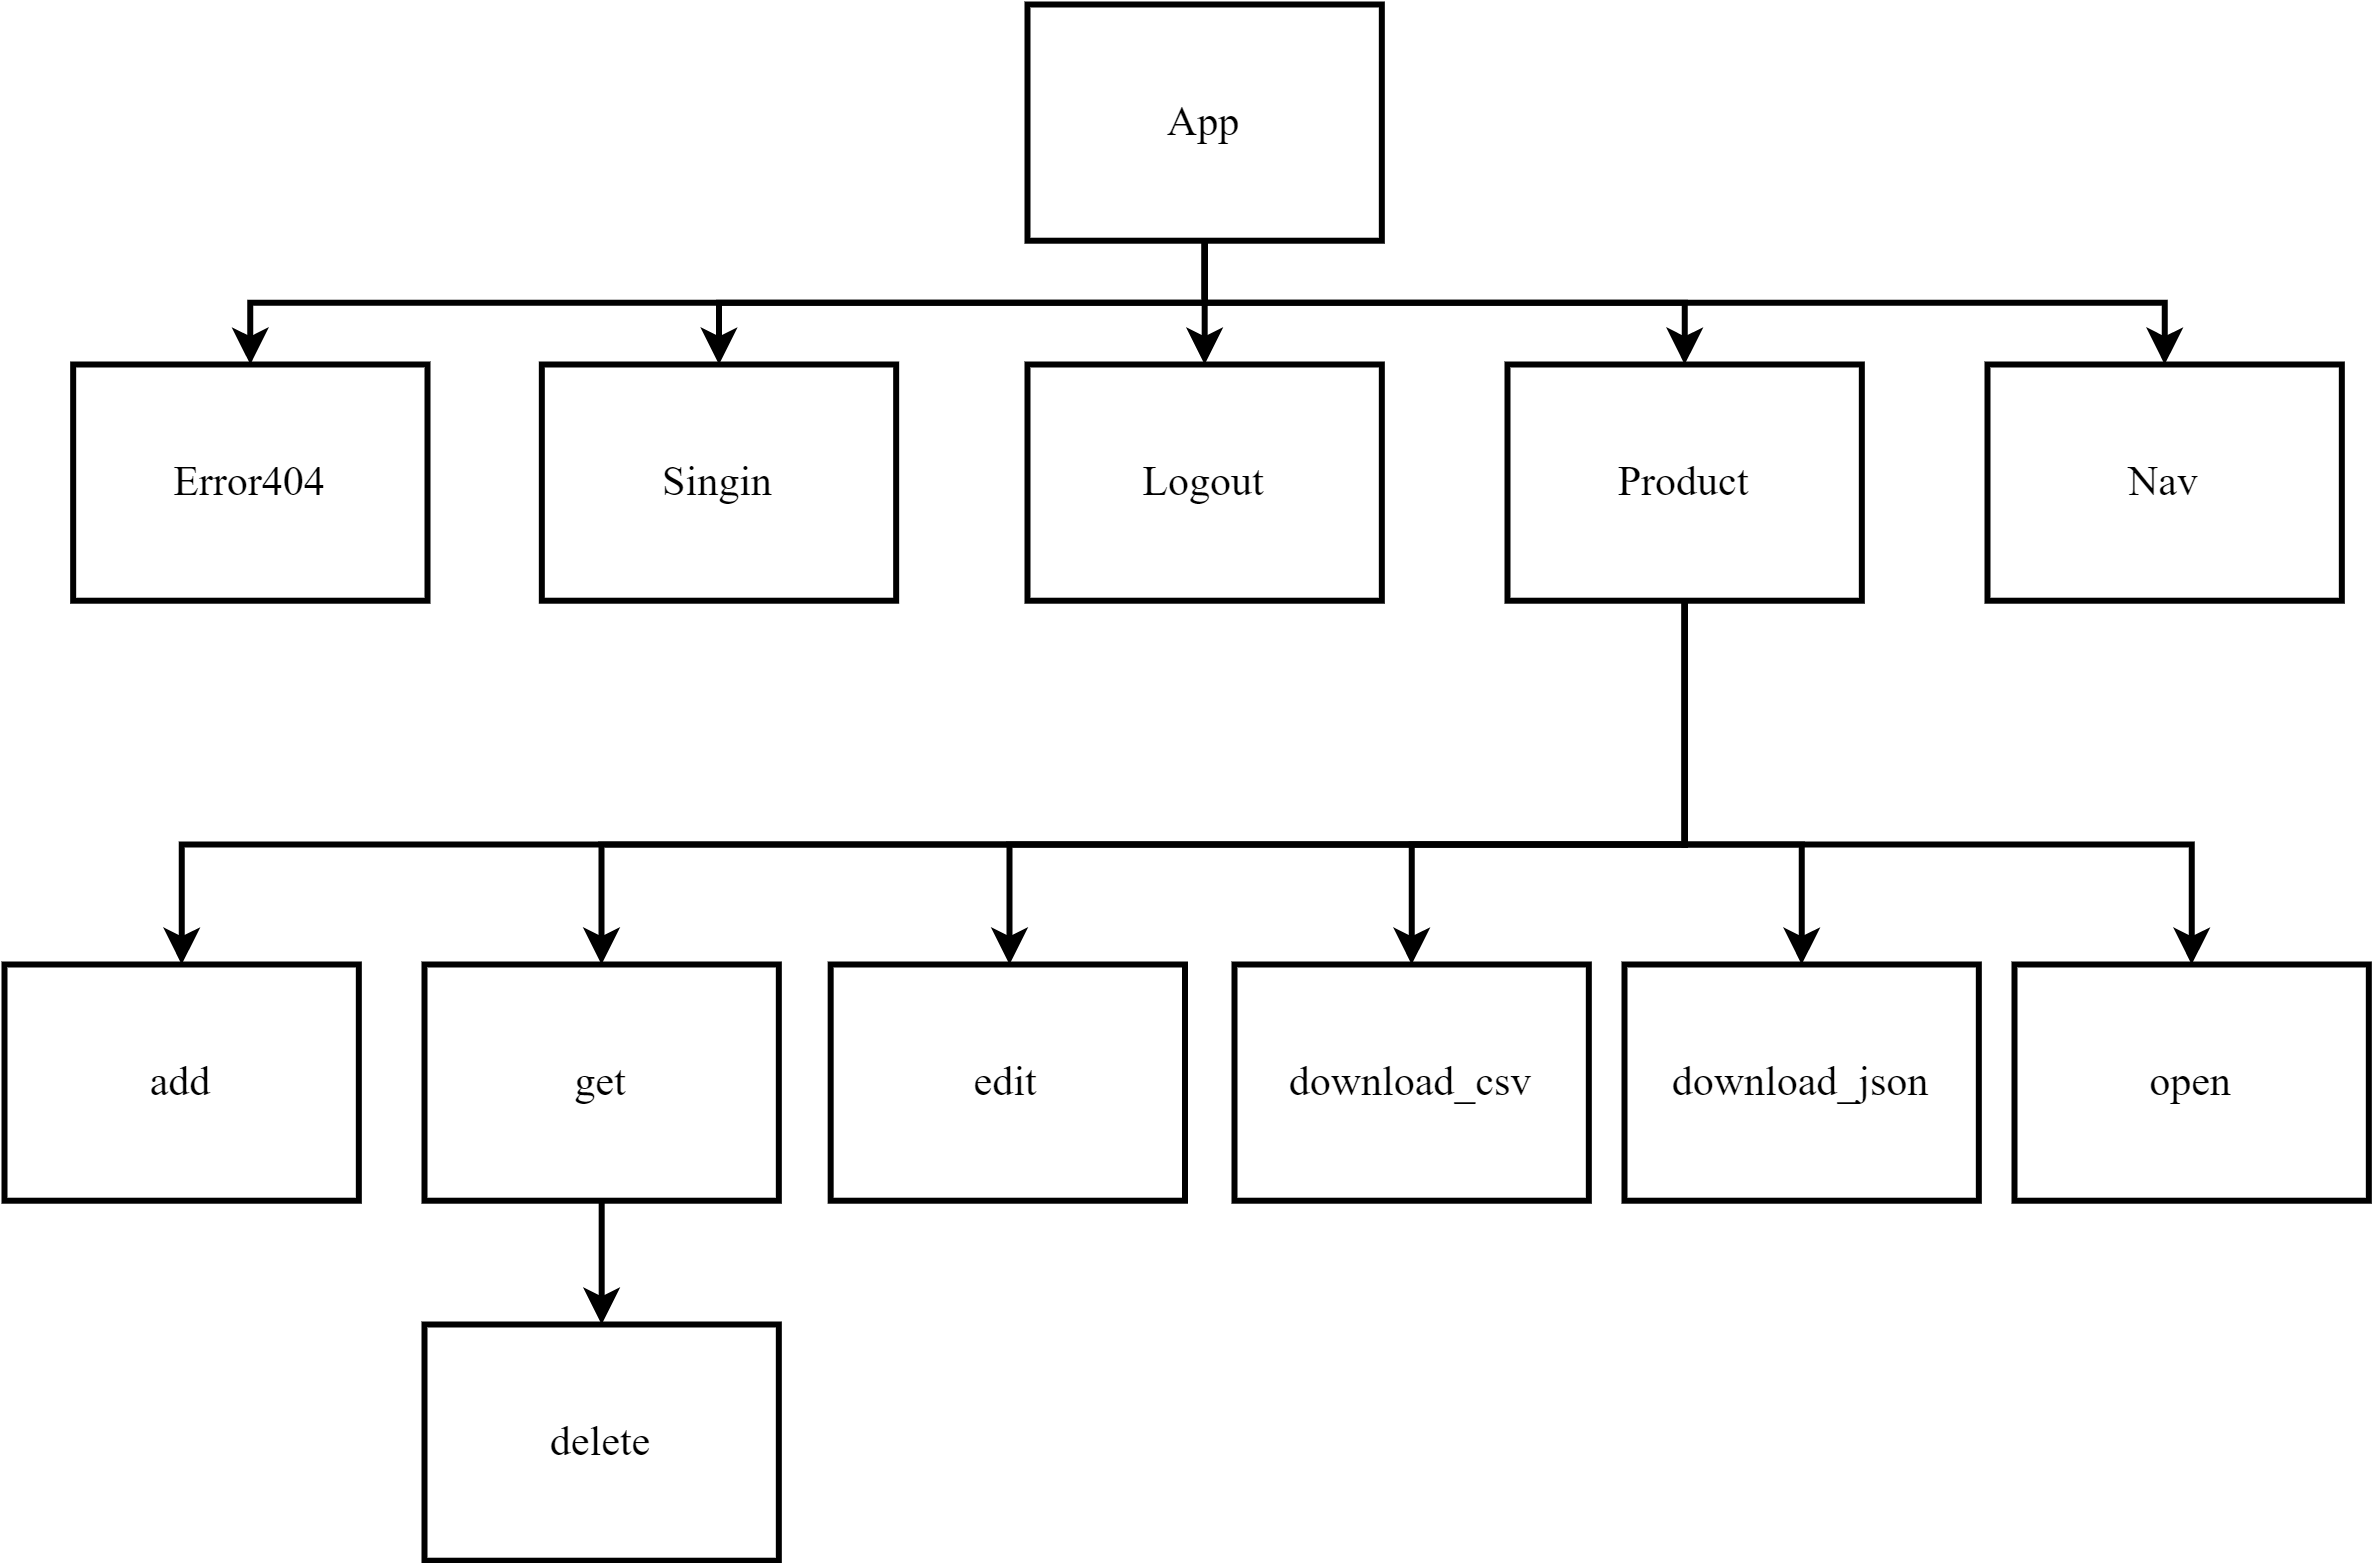
\includegraphics[width=13.7cm]
        {_assets/gpi_frontend_modules.png}
    \caption{Модули и подмодули для frontend}
    \label{fig:gpi_frontend_modules}
\end{figure}

\newpage

\subsubsection*{Иерархия модулей и подмодулей разрабатываемой программы для backend}

Информационная система включает в себя следующие модули на backend:

\begin{itemize}
    \item модуль авторизации;
    \item модуль добавления элементов в базу данных;
    \item модуль вывода элементов сортированных, инвертированных или по ID;
    \item модуль редактирования элемента по ID;
    \item модуль удаления элемента по ID.
\end{itemize}

Схема backend модулей изображена на
\textbf{рис. \ref{fig:gpi_backend_modules} (стр. \pageref{fig:gpi_backend_modules})}.

\begin{figure}[!htp]
    \centering
    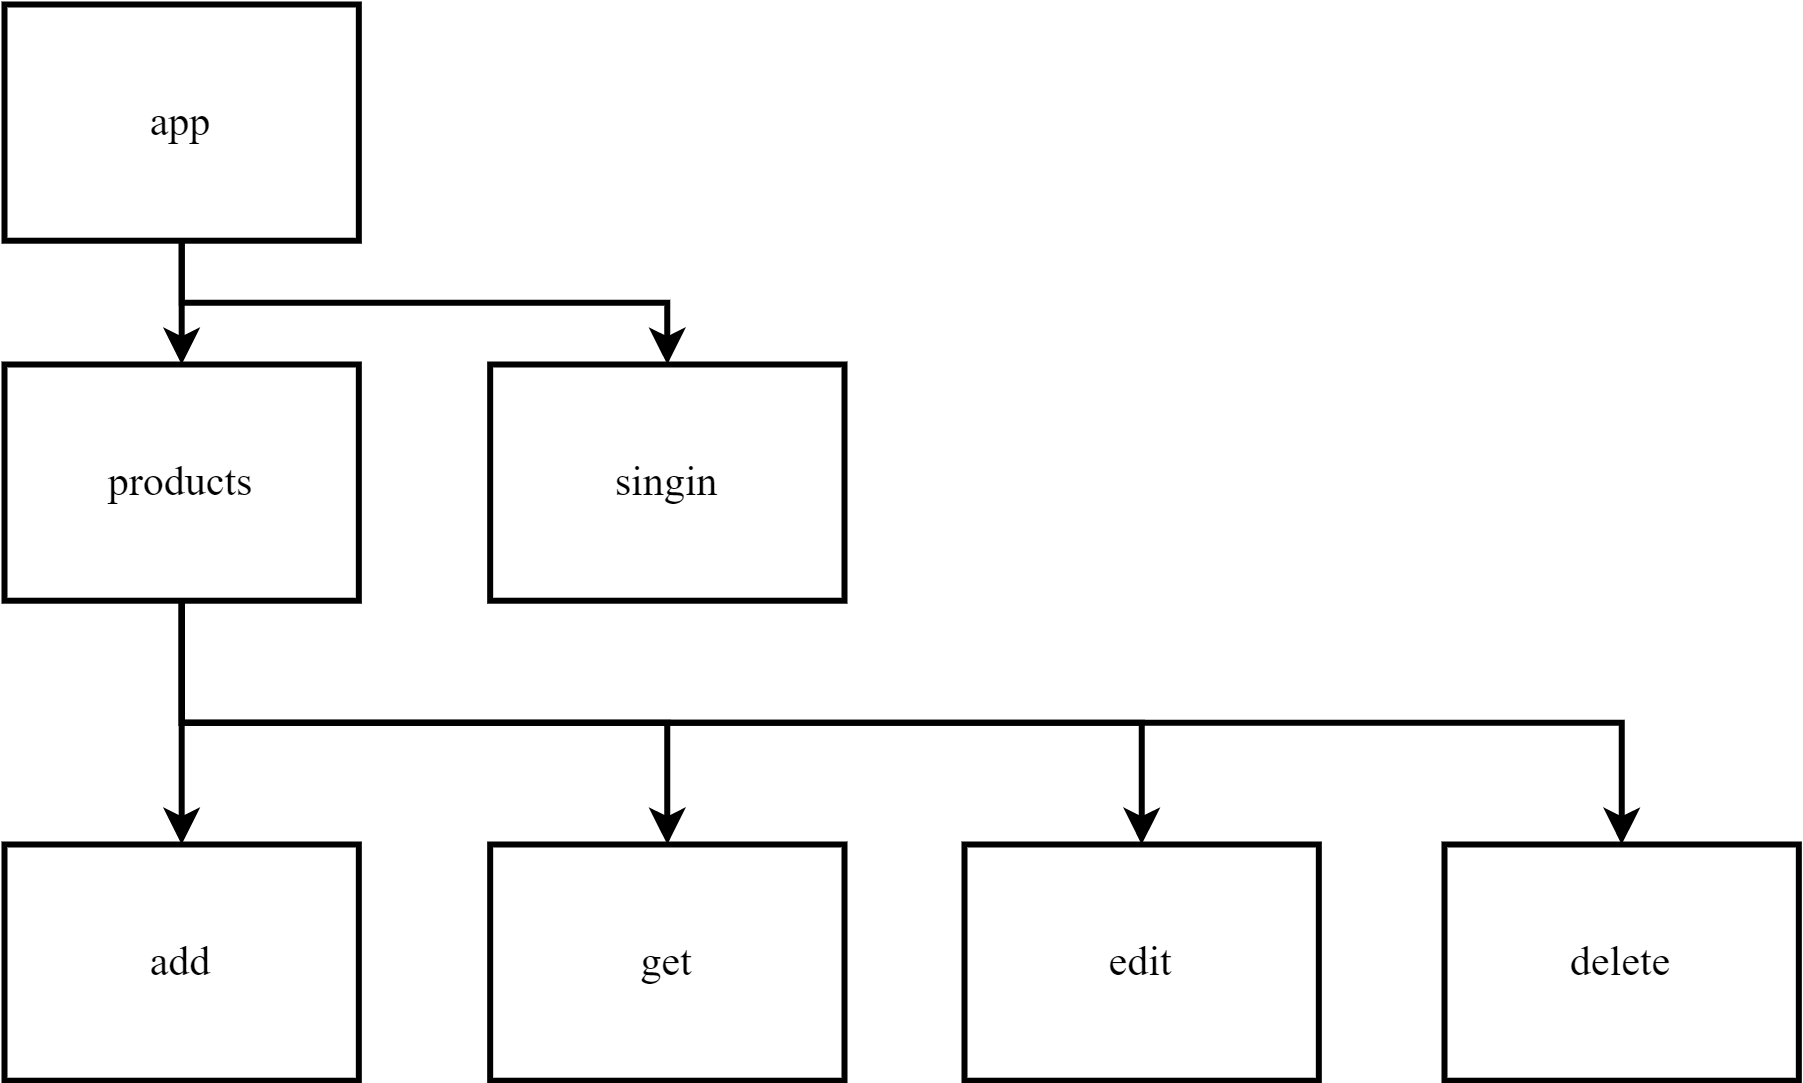
\includegraphics[width=12cm]
        {_assets/gpi_backend_modules.png}
    \caption{Модули и подмодули для backend}
    \label{fig:gpi_backend_modules}
\end{figure}

\subsection{Проект. Схема данных}

Трёхуровневая архитектура - архитектурная модель программного комплекса,
предполагающая наличие в нём трёх компонентов: клиента, сервера приложений
(к которому подключено клиентское приложение) и сервера баз данных.

Если мы посмотрим на данную архитектуру с позиции сайта.
То первый уровень можно считать браузером (frontend), с помощью которого посетитель заходит на сайт,
второй уровень - это Express server (backend), а третий уровень - это база данных MySQL.

Схема архитуктуры ПО изображена на
\textbf{рис. \ref{fig:gpi_client_server} (стр. \pageref{fig:gpi_client_server})}.

\begin{figure}[!htp]
    \centering
    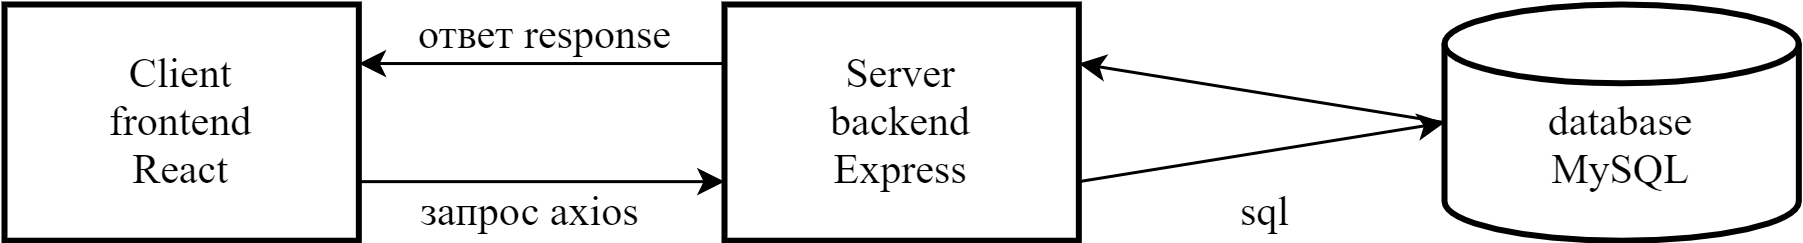
\includegraphics[width=16cm]
        {_assets/gpi_client_server.png}
    \caption{Схема архитектуры ПО}
    \label{fig:gpi_client_server}
\end{figure}

\subsection{Проектирование UI (макеты)}

Интерфейс будет содержать шапку сайта, которая в себе содержит навигацию (основные страницы).
Макет на \textbf{рис. \ref{fig:gpi_ui_menu} (стр. \pageref{fig:gpi_ui_menu})}.

В теле сайта на странице добавления будет находится форма,
через которую можно добавить поля в базу данных.

В теле сайта на странице вывода будет таблица с элементами из базы данных.
Макет на \textbf{рис. \ref{fig:gpi_ui_get} (стр. \pageref{fig:gpi_ui_get})}.

В теле сайта на странице редактирования будет находится форма,
через которую можно изменить поля в базе данных.

В теле сайта на странице открытия файла будет кнопка загрузки файла.

В теле сайта на странице сохранения файла CSV будет кнопка загрузки файла.

В теле сайта на странице сохранения файла JSON будет кнопка загрузки файла.

\begin{figure}[!htb]\centering
    \begin{minipage}{0.49\textwidth}
        \centering
        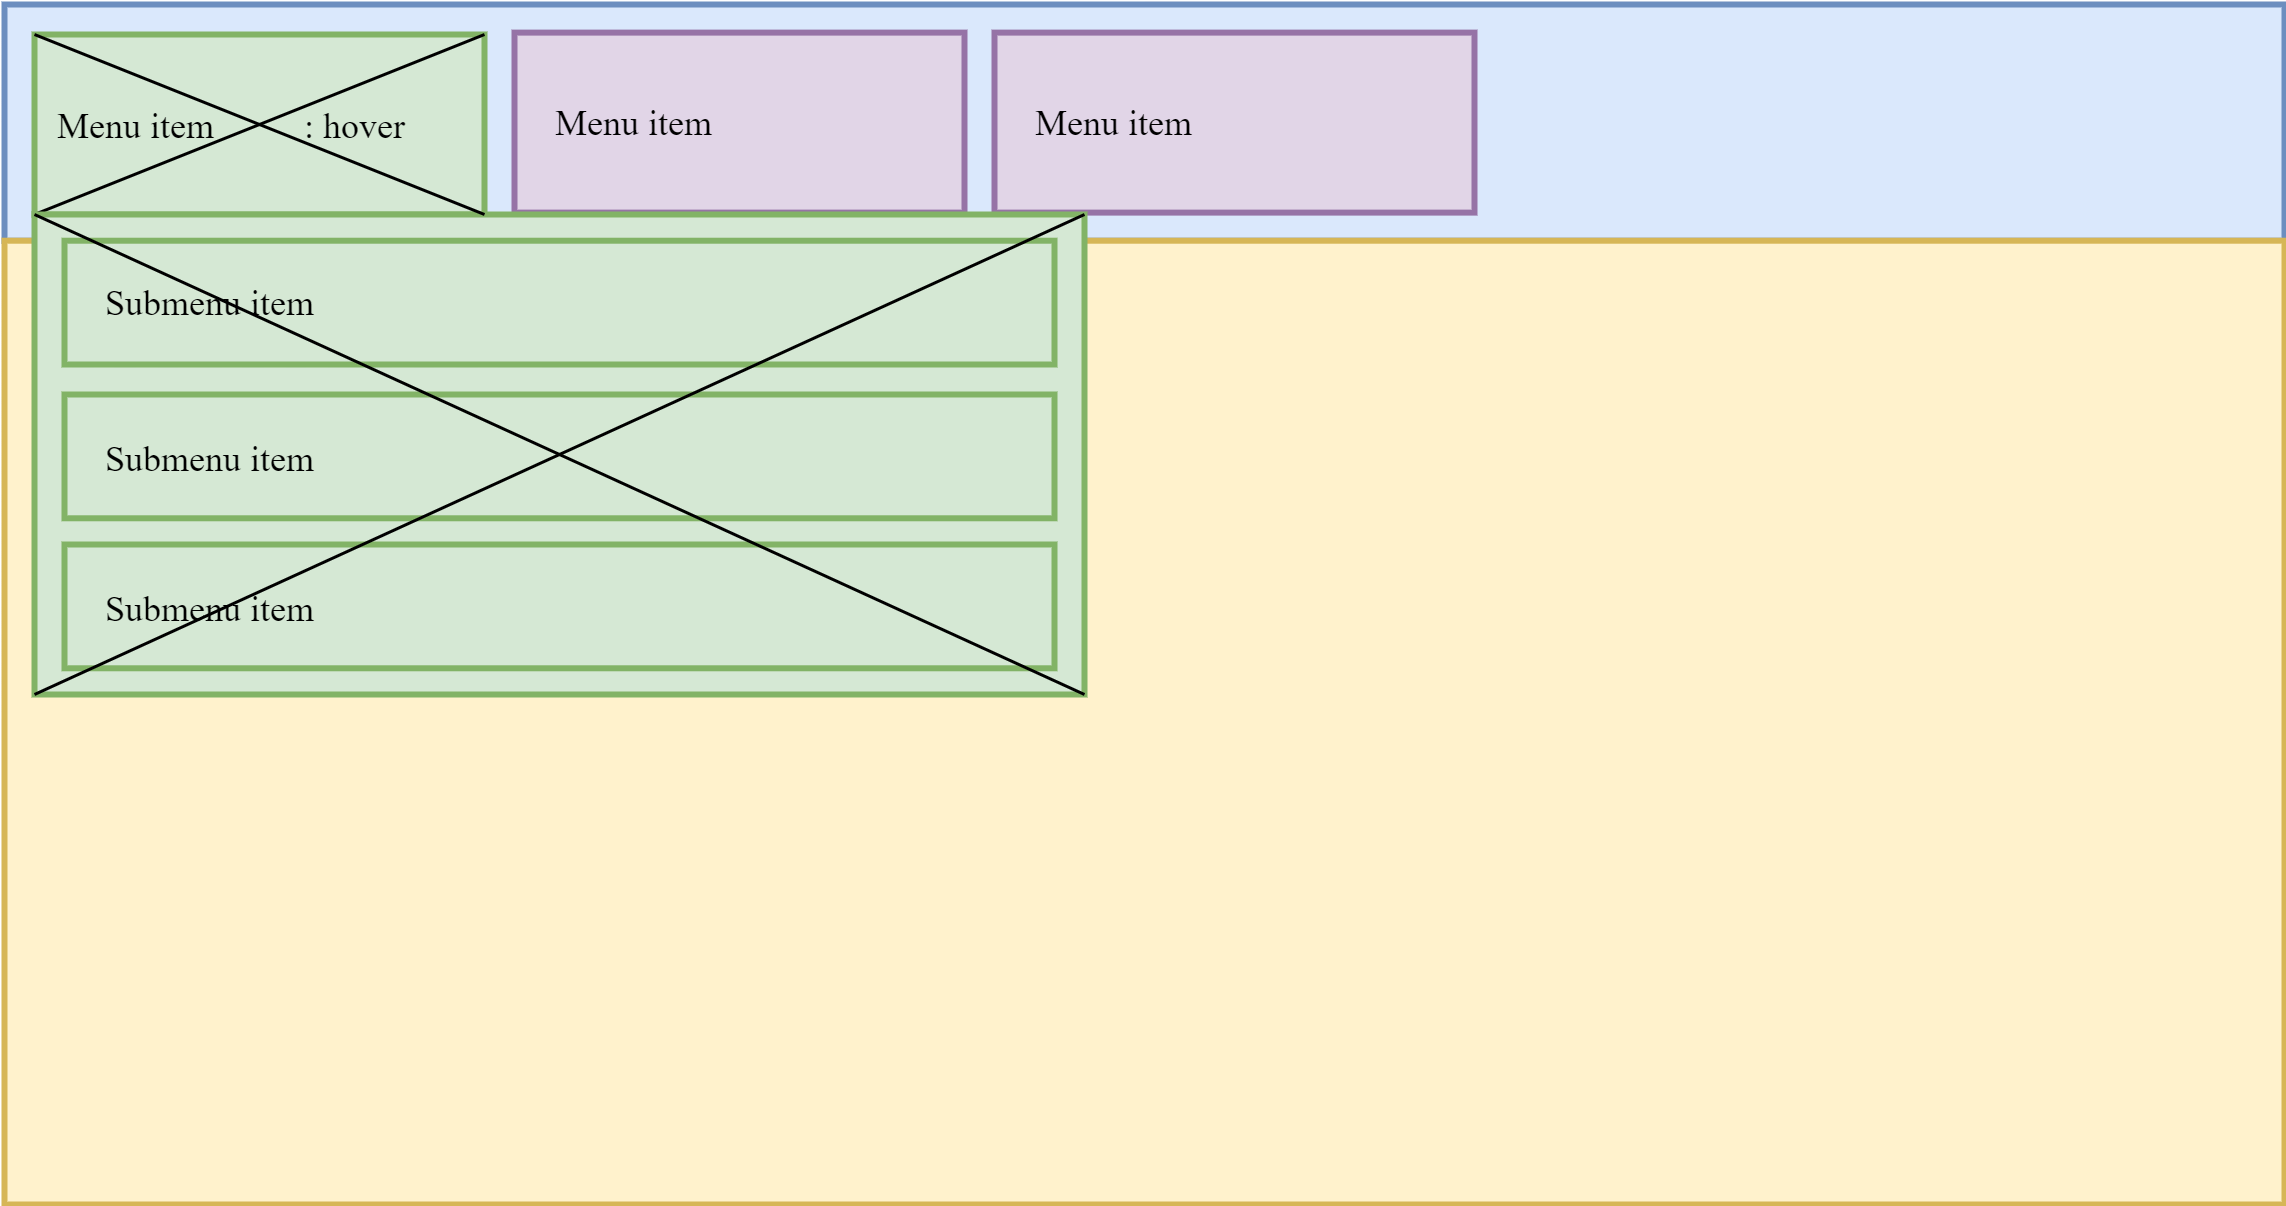
\includegraphics[width=0.99\linewidth]
            {_assets/gpi_ui_menu.png}
        \caption{Макет мeню}
        \label{fig:gpi_ui_menu}
    \end{minipage}
    \begin {minipage}{0.49\textwidth}
        \centering
        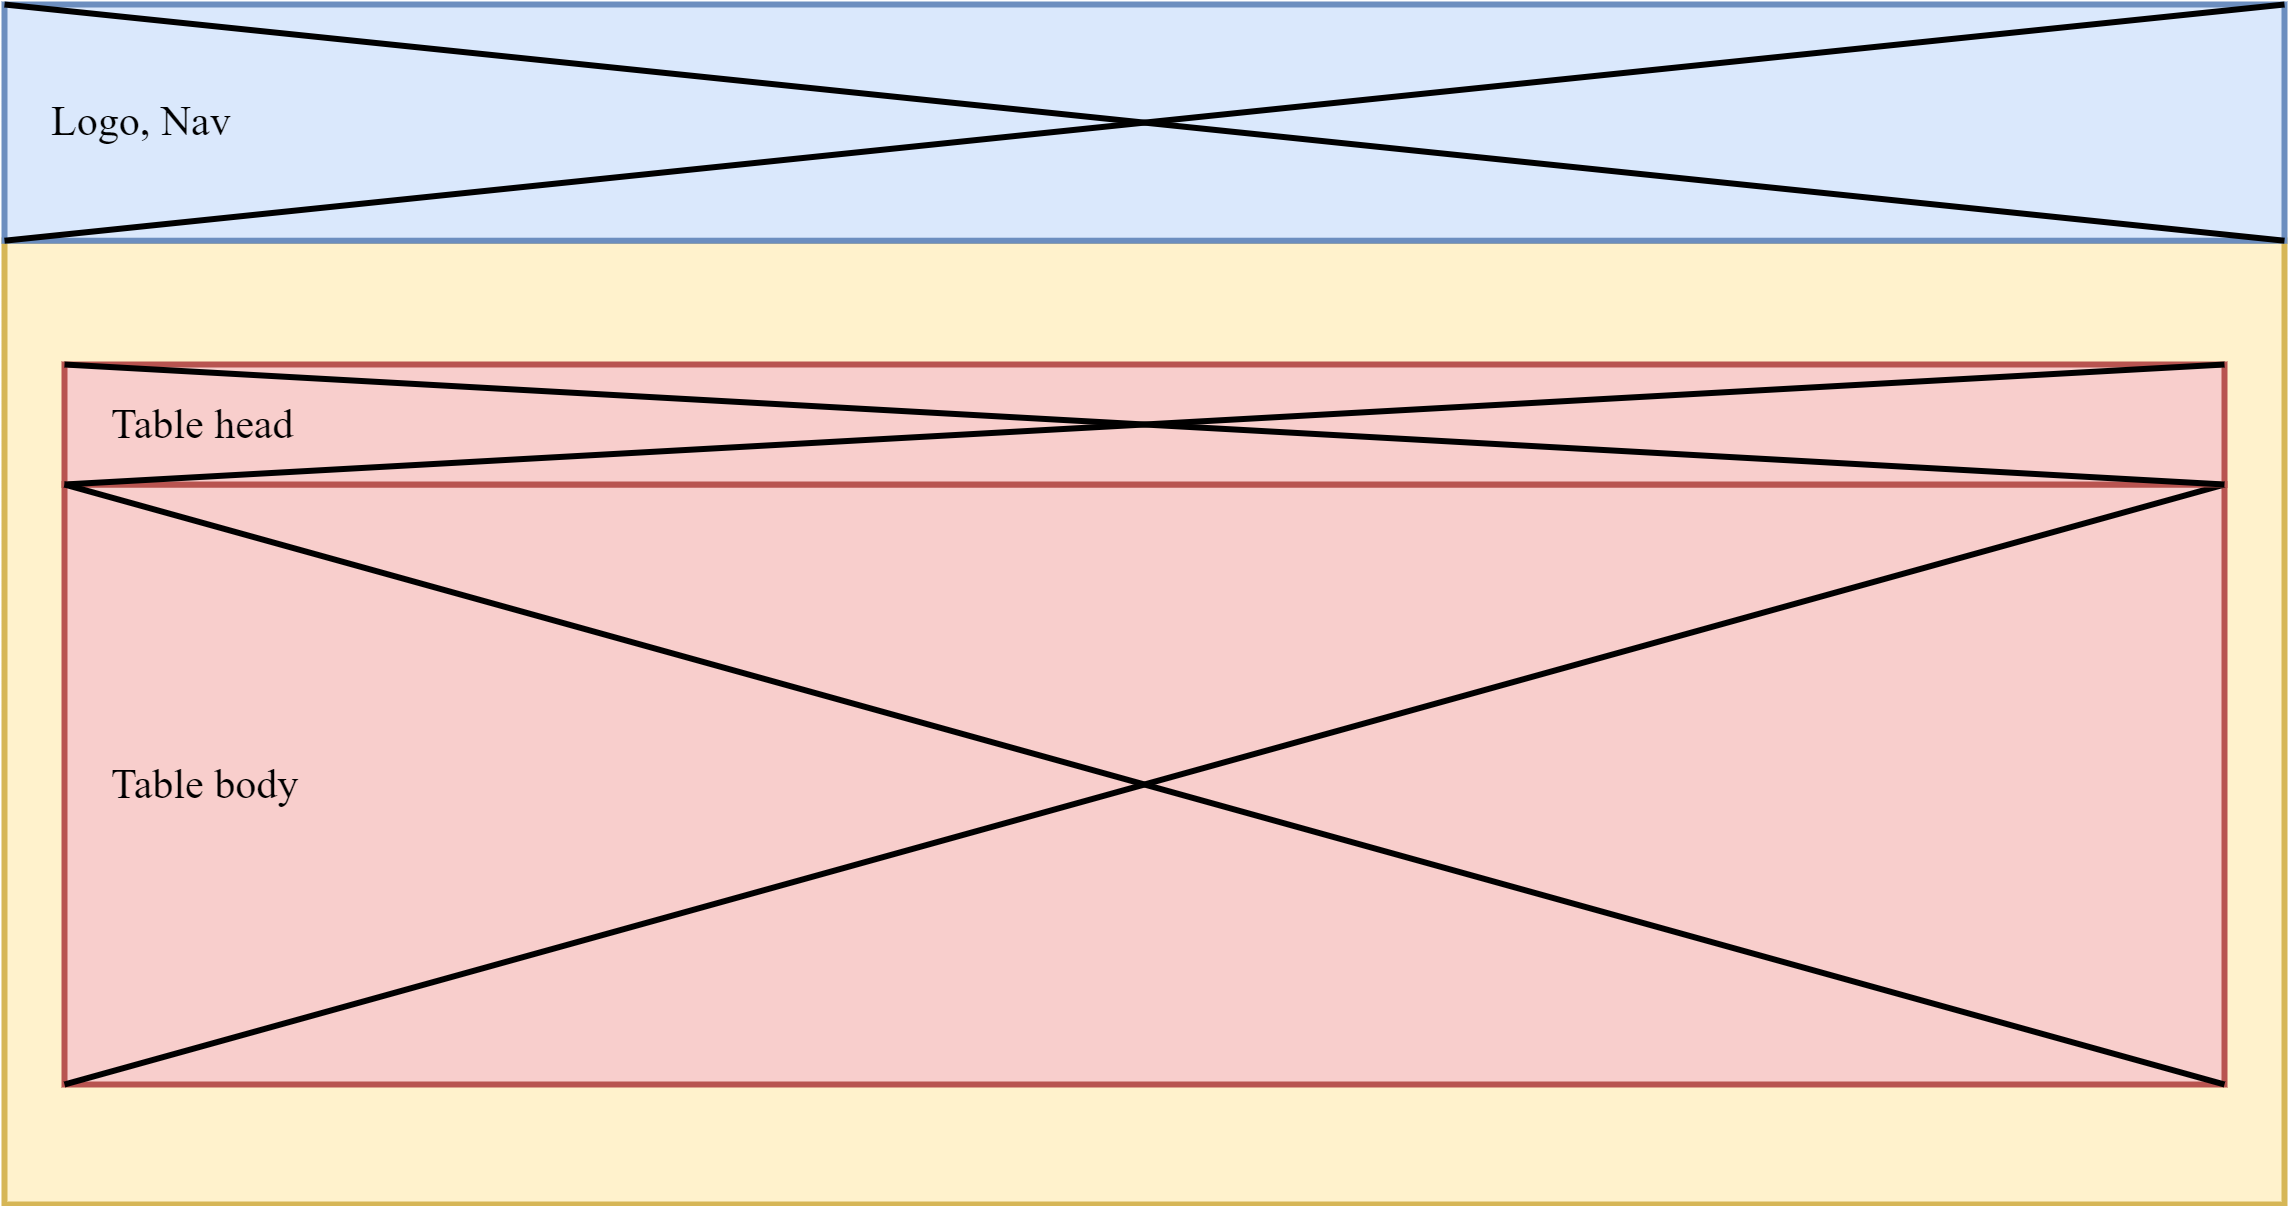
\includegraphics[width=0.99\linewidth]
            {_assets/gpi_ui_get.png}
        \caption{Макет страницы}
        \label{fig:gpi_ui_get}
    \end{minipage}
\end{figure}

\newpage
